\chapter{Algorytmy przetwarzania chmur punktów w systemach GIS}

\section{Pozyskiwanie danych}
Do pozyskiwania danych wykorzystuje się technologię LIDAR. Jest to nowoczesna metoda pozyskiwania informacji dotyczących wysokości terenu \cite{Marmol2003}. Efektem jej działania jest tzw “chmura punktów”, która uwzględnia wysokość nie tylko powierzchni ziemi, ale również drzew, budynków itp.

Dane zbierane są za pomocą aparatury umieszczonej w samolotach, na którą składają się odbiornik GPS służący do określania pozycji, czujnik INS pozwalający na określenie aktualnego przechyłu pojazdu oraz laser
LRF mierzący odległość \cite{WBPW2012}. Laser emituje wiązkę w kierunku ziemi. Na podstawie czasu jaki minął między emisją wiązki a jej odczytem, określana jest odległość między aparaturą a badanym punktem.
Jednocześnie zapisywane jest położenie skanera, co pozwala umieścić punkt w układzie odniesienia (np: WGS 84). Poza odległością (która przekłada się na wysokość punktu nad powierzchnią) zbierane są też inne
informacje takie jak \cite{chen2014}:
\begin{itemize}
\item Intensywność (zwana również amplitudą) - Intensywność wskazuje na charakterystykę odbicia od powierzchni, tym samym mogąc posłużyć do analizy typu powierzchni \cite{yunfei2008};
\item Różnica w wysokości pierwszego i ostatniego odbicia - Wiązka laserowa może w pewnym stopniu penetrować napotkane powierzchnie. W sytuacji, w której część wiązki spenetruje napotkaną powierzchnię,
    wysokość powiązana z pierwszym odbiciem będzie inna, niż wysokość powiązana z ostatnim odbiciem. Z drugiej strony, dla nawierzchni twardych, jak dachy czy ulice, wartości te dla wszystkich odbić będą 
    takie same \cite{chen2014};
\item Różnica w intensywności pierwszego i ostatniego odbicia - Może być wykorzystana analogicznie do różnicy w wysokości \cite{chen2014}.\ldots
\end{itemize}

\begin{figure}[h!]
\centering
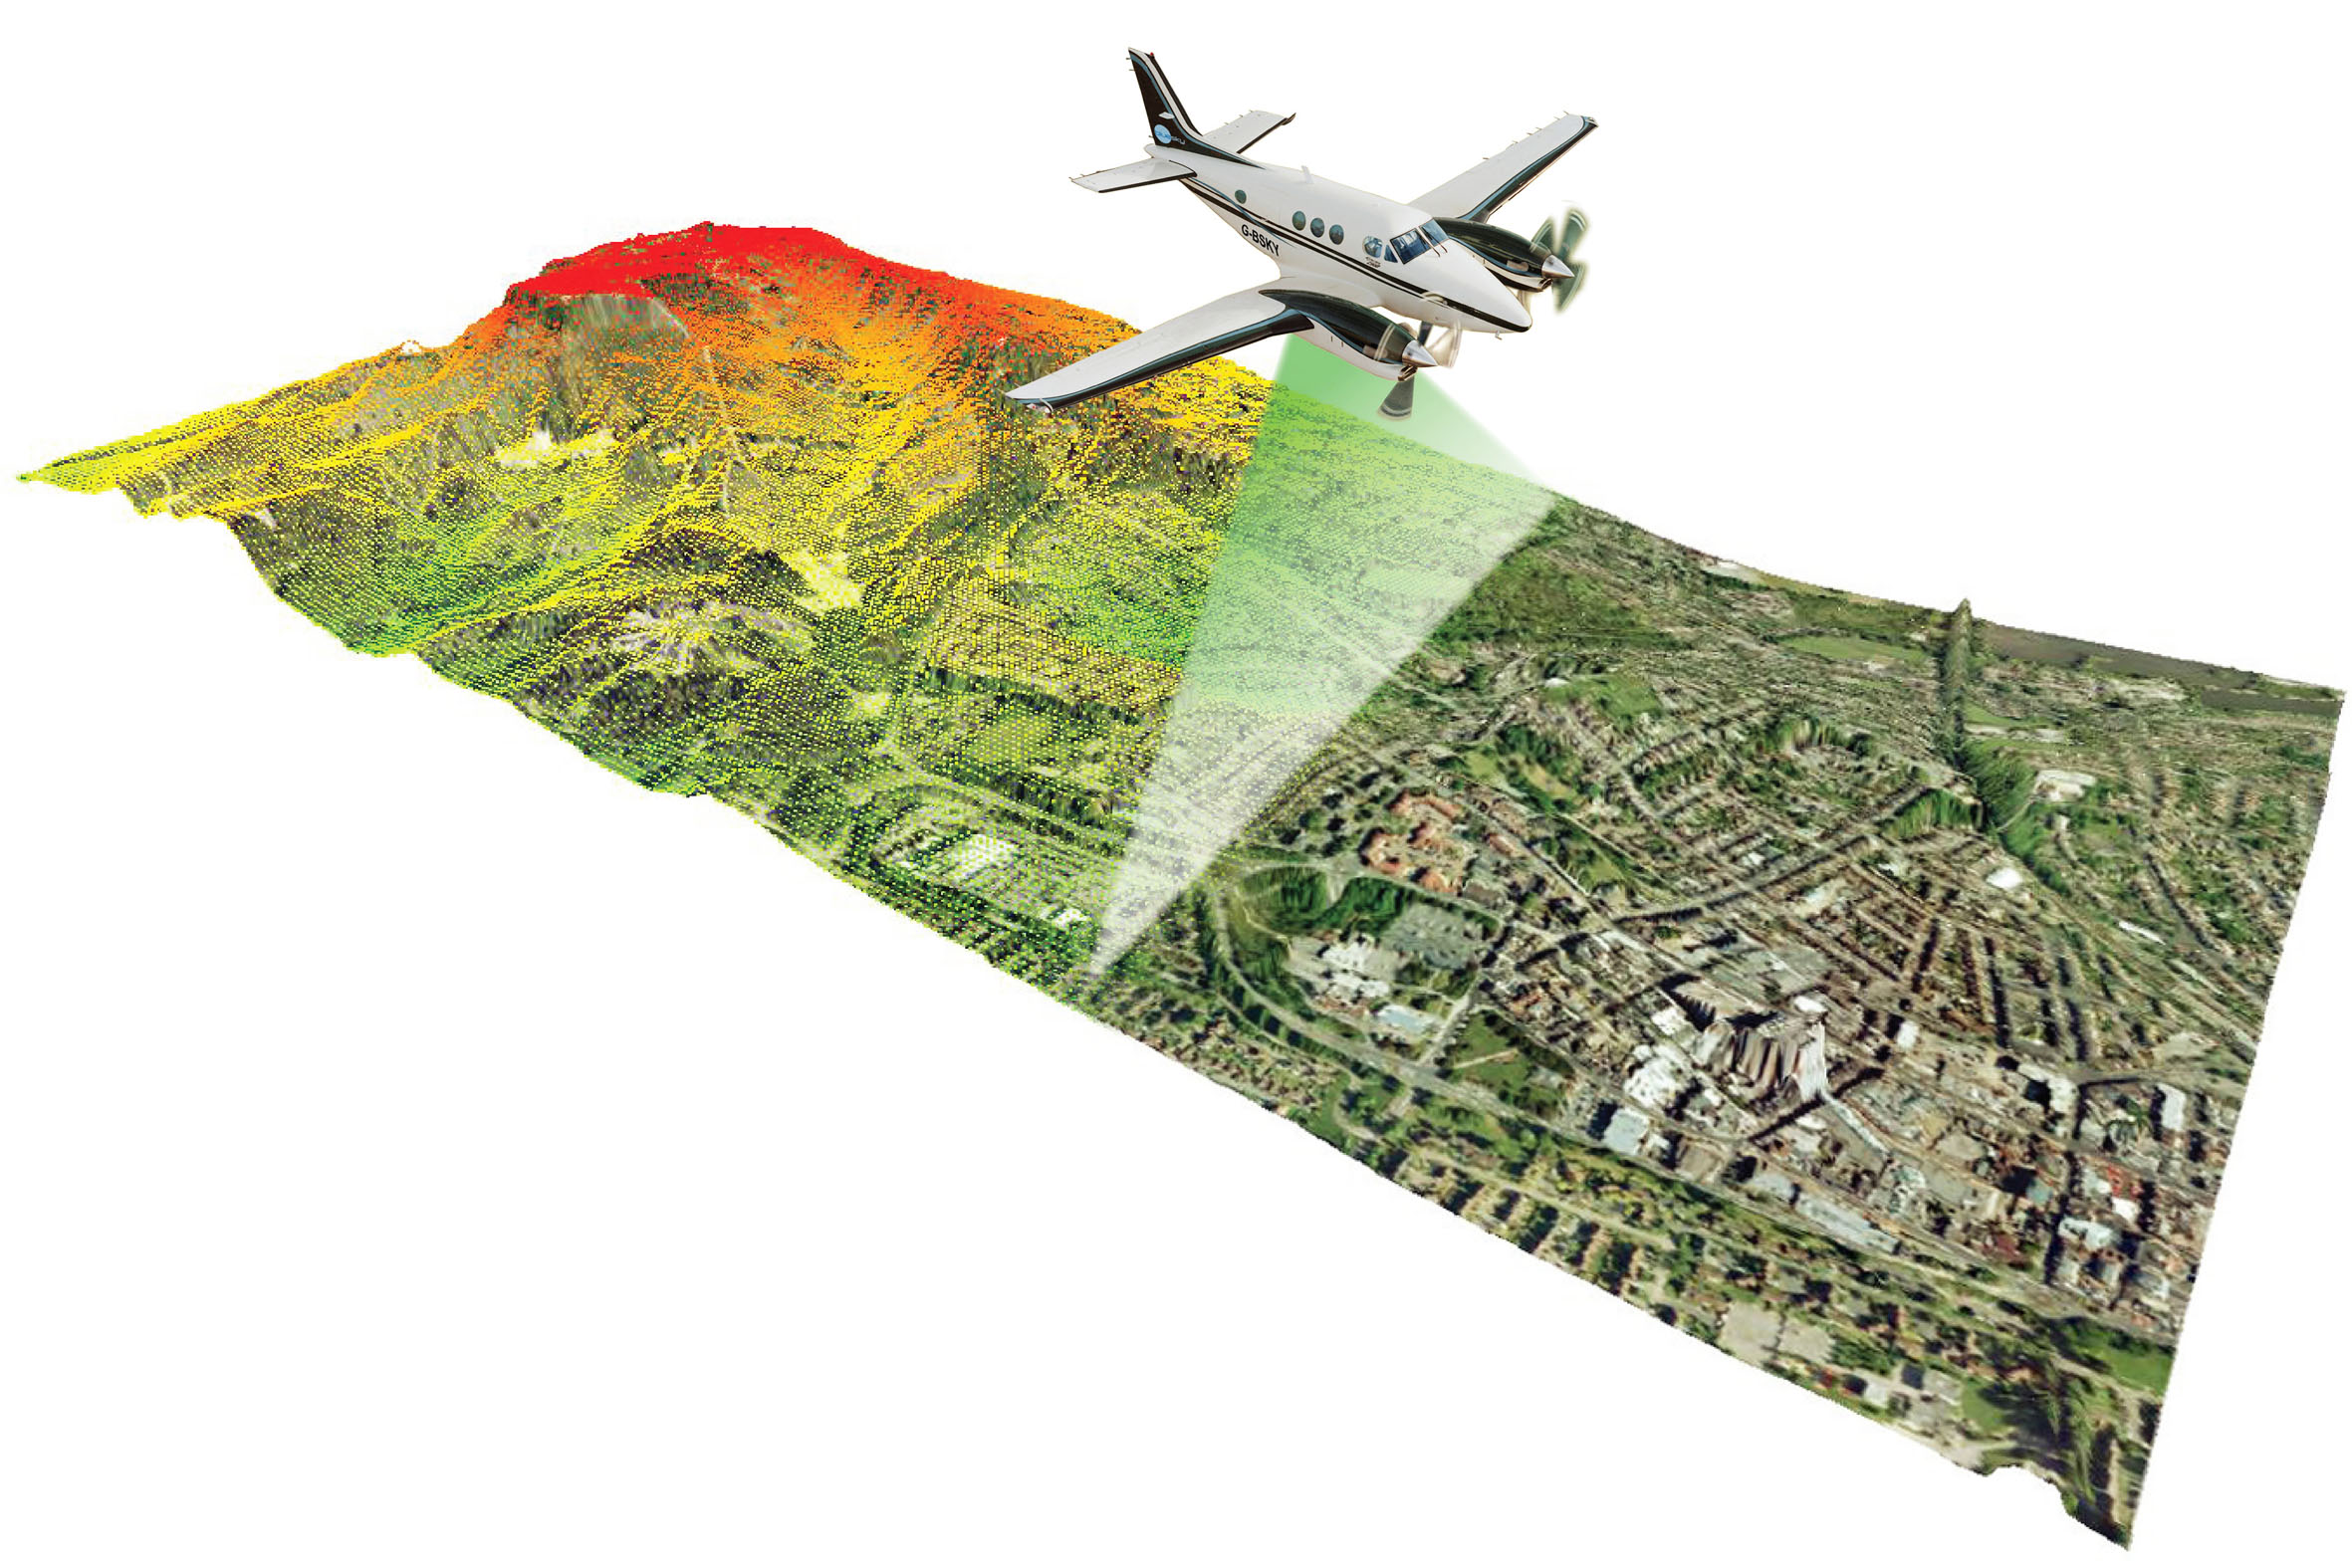
\includegraphics[width=0.9\textwidth]{img/LIDAR.jpg}
\caption{Schematycznie przedstawiony nalot podczas zbierania danych LIDAR}
\label{fig:lidar}
\end{figure}

Na rysunku \ref{fig:lidar} przedstawiono w sposób schematyczny jak przebiega pobieranie danych. Samolot podczas nalotu pobiera dane wzdłuż pewnego odcinka prostopadłego do kierunku lotu, z których następnie powstaje chmura punktów, której wizualizację również przedstawiono na rysunku.

\section{Opis wybranych algorytmów}

W poniższym rozdziale zostaną opisane istniejące algorytmy przetwarzania danych w postaci chmury punktów w systemach GIS.

\subsection{Triangulacja Delaunay'a}

\subsubsection{Definicja}
Triangulacja Delaunay'a jest reprezentacją chmury punktów w postaci nieregularnej siatki trójkątów TIN (z ang. Triangulated Irregular Network).
Jej cechą szczególną jest fakt, iż żaden z punktów nie leży wewnątrz okręgu opisanego na dowolnym trójkącie \cite{Lee1980}. Podział ten ma tę własność, że maksymalizuje najmniejszy kąt spośród 
wszystkich trójkątów należących do triangulacji. Na rysunku \ref{fig:triangulacja} przedstawiono przykładową triangulacje.

\begin{figure}[h!]
    \centering
    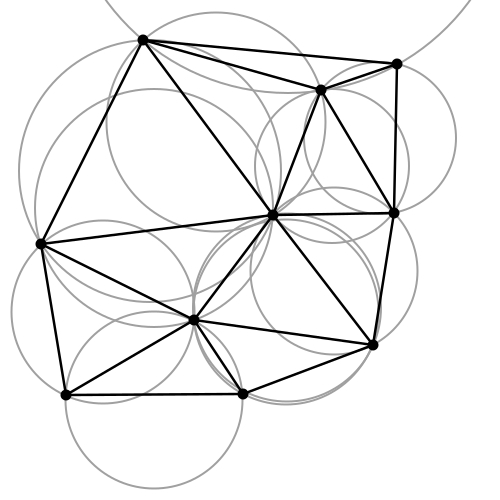
\includegraphics[width=0.5\textwidth]{img/triangulacja.jpg}
    \caption{Triangulacja Delaunay z zaznaczonymi okręgami opisanymi na trójkątach}
    \label{fig:triangulacja}
\end{figure}

\subsubsection{Aplikacje}
Triangulacja Delaunay'a jest często wykorzystywana przy przetwarzaniu danych LIDAR. Dzięki stosowaniu filtracji może służyć do oddzielania poszczególnych zbiorów punktów od siebie \cite{koziol2007} bądź też do znajdywania łamanej otaczającej zadany zbiór punktów \cite{website:HumanGeoBlog}. Istnieje wiele implementacji algorytmu pozwalającego na przetworzenie chmury punktów do postaci siatki trójkątów \cite{Lee1980,Dwyer1987,jiang2010}. W artykule \cite{Lee1980} opisano dwa algorytmy tworzenia takiej siatki - dziel i zwyciężaj oraz tribuild. Pierwszy z nich o złożoności obliczeniowej $O(N log N)$ rekurencyjnie dzieli zbiór punktów pośrednich na mniejsze zbiory, w nich dokonuje triangulacji a następnie łączy je. Drugi z nich o złożoności obliczeniowej $O(N^{3/2})$ zakłada znajomość prostokąta który otacza zadany zbiór punktów. Prostokąt ten jest dzielony na mniejsze, a następnie dla każdego mniejszego prostokąta:

\begin{algorithmic}
    \For {punkt P w punktach należących do prostokąta}
    \If {P jedyny punkt w prostokącie}
        \State połącz punkt z wierzchołkami prostokąta
    \Else
        \State dodaj krawędzie, aby nie zniszczyć triangulacji
    \EndIf
    \EndFor
\end{algorithmic}

Przykładowe kolejne etapy tak przeprowadzonej triangulacji pokazano na rysunku \ref{fig:iter_triangulacja}.

\begin{figure}[h!]
    \centering
    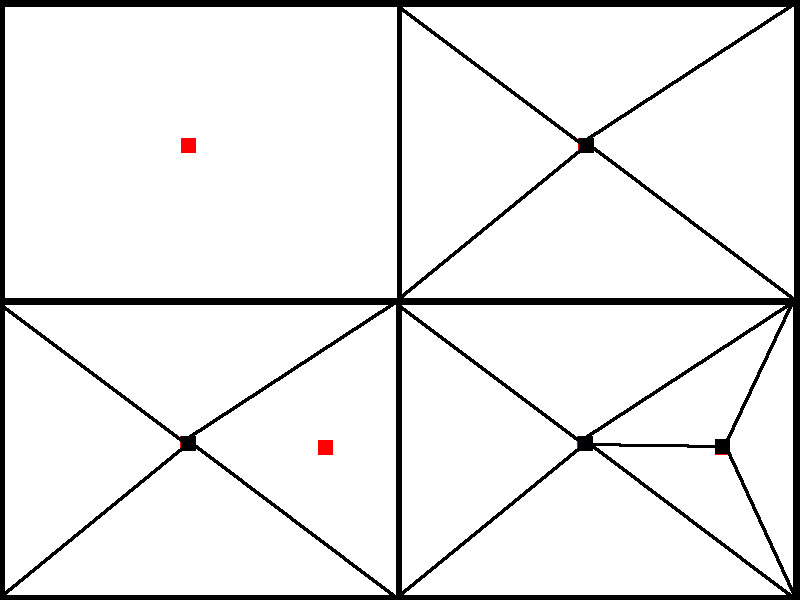
\includegraphics[width=0.5\textwidth]{img/iter_triangulacja.jpg}
    \caption{Iteracyjna triangulacja}
    \label{fig:iter_triangulacja}
\end{figure}

W 1987 Dwayer zaproponował szybszy algorytm dziel i zwyciężaj, o zakładanej złożoności $O(N log log N)$, jednak w pesymistycznym przypadku dalej będzie to $O(N log N)$  \cite{Dwyer1987}. Powstały też nowsze algorytmy pozwalające na stworzenie triangulacji. W artykule \textsl{An efficient algorithm for constructing Delaunay triangulation} autorzy zwracają uwagę, że w większości algorytmów szybko tworzy się siatkę a następnie dużo czasu poświęca się na lokalne optymalizacje, co skutkuje zwiększoną złożonością obliczeniową. Dzięki zaproponowaniu reguły prawej dłoni, udało im się znacząco zmniejszyć ilość obliczeń potrzebnych do przeprowadzenia lokalnych optymalizacji, tym samym proponowany algorytm ma złożoność na poziomie $O(N)$ \cite{jiang2010}.

\subsection{Maszyny wektorów nośnych}

\subsubsection{Definicja} 

Maszyny wektorów nośnych SVN (z ang. \textit{support vector machine}) pozwalają na rozwiązanie tzw. problemu klasyfikacji. Definicja problemu brzmi następująco: dla pewnej przestrzeni $\Omega$ zawierającej wektory danych x, należące do dwóch klas
$\Omega = \{(x_{i}, c_{i}) | x_{i} \in R^p, c_{i} \in \{-1,1\}\}$
należy znaleźć klasyfikator który podzieli tę przestrzeń na dwa rozłączne obszary jak najlepiej odpowiadające klasom $\{-1, 1\}$ \cite{stefanowski2010}. Do rozdzielenia zbioru na dwa służy tzw. liniowa funkcja separująca (lub jej uogólnienie - hiperpłaszczyzna dla przypadków n-wymiarowych), która wyznacza podział przestrzeni na dwa podobszary.

\begin{figure}[h!]
    \begin{subfigure}[b]{0.33\textwidth}
        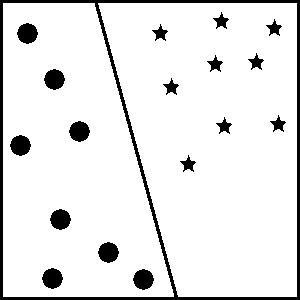
\includegraphics[width=\linewidth]{img/granica_1.jpg}
    \end{subfigure}%
    \begin{subfigure}[b]{0.33\textwidth}
        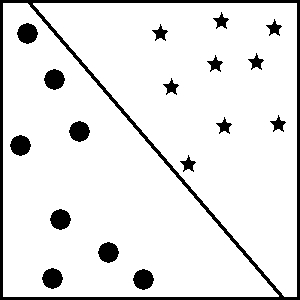
\includegraphics[width=\linewidth]{img/granica_2.jpg}
    \end{subfigure}%
    \begin{subfigure}[b]{0.33\textwidth}
        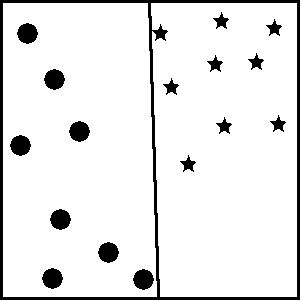
\includegraphics[width=\linewidth]{img/granica_3.jpg}
    \end{subfigure}
    \caption{Różne przykłady liniowej separacji}
    \label{fig:liniowa_separacja}
\end{figure}

Na rysunku \ref{fig:liniowa_separacja} przedstawiono różne poprawne sposoby separowania tego samego zbioru. Można w szczególności wyróżnić pary hiperpłaszczyzn $b_{i1}$ oraz $b_{i2}$, będących równoległych do 
siebie, powstałych poprzez przesuwanie jednej hiperpłaszczyzny od punktu granicznego pierwszego zbioru do punktu granicznego drugiego zbioru (rysunek \ref{fig:rownolegla_separacja}).

\begin{figure}[h!]
    \centering
    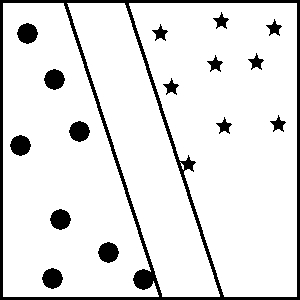
\includegraphics[width=0.33\textwidth]{img/granica_rownolegla.jpg}
    \caption{Równoległe hiperpłaszczyzny}
    \label{fig:rownolegla_separacja}
\end{figure}

Odległości pomiędzy hiperpłaszczyznami $b_{i1}$ oraz $b_{i2}$ nazywamy marginesem klasyfikatora liniowego. Maszyny wektorów nośnych znajdują taką hiperpłaszczyznę, która maksymalizuje margines. Szukamy więc hiperpłaszczyzny spełniającej warunki:

\begin{equation}
    w*x + b =0
\end{equation}

gdzie $w$ i $b$ są parametrami modelu. Wtedy przynależność do klas można wyrazić jako:

\begin{displaymath}
    y = \left\{ \begin{array}{ll}
        1 & \textrm{$w*x+b>0$}\\
        -1 & \textrm{$w*x+b<0$}\\
    \end{array} \right.
\end{displaymath}

Parametry $w$ i $b$ należy wyznaczać tak, aby maksymalne marginesy $b_{i1}$ i $b_{i2}$ były miejscem geometrycznym punktów $x$ spełniających warunki:
\begin{eqnarray}
    b_{i1} \quad w*x + b =1 \\
    b_{i2} \quad w*x + b =-1
\end{eqnarray}

\subsubsection{Aplikacje}

Możliowości wykorzystania maszyn wektorów nośnych do przetwarzania chmury punktów nasuwają się same - możliwe jest chociażby przydzielanie punktów do klas drzew i budynków \cite{xwang2011}. Istnieje wiele 
różnych przykładów na wykorzystanie SVN do przetwarzania chmur punktów \cite{xwang2011,li2013,david2015}. We wszystkich z nich część punktów pomiarowych jest wykorzystywana jako dane uczące.
Dla tych punktów operator ręcznie przydziela je do jednej z klas \cite{xwang2011}. Następnie na podstawie tych punktów możliwe jest określenie najlepszej hiperpłaszczyzny, jak opisano w sekcji \textit{definicja}.
W pracy z 2011r. wykorzystano tzw. niezbalansowane maszyny wektorów nośnych USVN (z ang. \textit{unbalanced support vector machines}) do rozróżnienia drzew i budynków \cite{xwang2011}.
Do analiz wykorzystano zdjęcia satelitarne oraz dane pochodzące z LIDARa - za pomocą tych dwóch źródeł stworzono wektory $x$ składające się z wysokości $Z$, wariancji wysokości $sZ$, różnice wysokości $hZ$,
pochodne 3-go rzędu wzdłuż osi X i Y - odpowiedno $dX$ i $dY$ - oraz wartość koloru RGB ze zdjęcia satelitarnego. 
W pracy \textit{Land classification from LiDAR full-waveforms based on multi-class support vector machines} wykorzystano SVM do przypisywania punktów do więcej niż dwóch klas \cite{li2013}. 
W innej pracy z 2015 równierz wykorzystano SVM do podziału zbioru na więcej niż dwie klasy \cite{david2015}. Analiza to posłużyła do zmierzenia powierzchni namorzyn na Filipinach. 
W tym przypadku do stworzenia wektorów $x$ wykorzystano numeryczny model powierzchmi DSM, numeryczny model terenu DTM, model wysokościowy CHM, średnią intensywność oraz ilość odbić. Co ciekawe, na podstawie
ilości odbić można określić gatunek drzewa \cite{Sasaki2012}.

\subsection{Analiza obrazu oparta obiektowo}

\subsubsection{Definicja}

Analiza obrazu oparta obiektowo OBIA (z ang. \textit{Object – based image analysis}) jest stosunkowo nową metodą \cite{burnett2003} służącą do przetwarzania obrazów. W przeciwieństwie do tradycyjnych metod przetwarzania, 
nie analizuje pojedynczych pikseli, lecz całe ich grupy, zwane obiektami. Ma to przypominać sposób, w jaki ludzie rozróżniają obiekty na zdjęciach. Jeżeli zdjęcia dotczą powierzchni ziemi (takie jak zdjęcia 
satelitarne) wyróżnia się wtedy metodę geograficznej analizy obrazu oparte obiektowo GEOBIA (z ang. \textit{Geographic Object-based Image Analysis}). Jako że tematyka całej pracy dotyczy systemów GIS,
w dalszej części będzie opisywana ten szczególny przypadek OBIA.

Metoda ta składa się z dwóch etapów. w Pierwszym z nich grupuje się podobne piksele (np. pod względem koloru) w obiekty prymitwne (prymitywy). Prymitywy służą następnie do konstruowania bardziej złożonych 
struktur, odpowiadających rzeczywistym obiektom takim jak jeziora czy drogi \cite{Blaschke2014}.  Budowanie obiektów może odbywać się stopniowo na poziome wielu wartstw, jak przedstawiono na rysunku
\ref{fig:poziomy_struktury}.

\begin{figure}[h!]
    \centering
    \includegraphics[width=0.5\textwidth]{img/obiekowa_analiza.png}
    \caption{Podział obrazu na piksele i obiekty}
    \label{fig:poziomy_struktury}
\end{figure}

\subsubsection{Aplikacje}
Metoda ta jest szeroko używana do analizy danych pochodzących ze skanowania laserowego. Jest wykorzystywana do klasyfikowania terenów miejskich \cite{zhou2013,chen2014},
wykrywania zmian powierzchni lasu \cite{zhang2014} oraz do wspomagania zarządzania terminalem kontenerowym \cite{tiede2015}. W tym ostatnim wykorzystano technikę OBIA do dokładnego określania miejsca położenia
kontenerów. Jest to zadanie o tyle łatwiejsze, iż wielkość kontenerów jest znana i podana jako norma ISO 668. Do celów analizy stworzono model DTM na podstawie danych LIDAR. Następnie do wykrywania
umiejscowie kontenerów wykorzystano dane LIDAR (pochodzące z jednego nalotu) oraz wykonywane częściej zdjęcia. Efektem jest model 3D nabrzeża.

Na polu analizy i klasyfikacji terenów miejskich metoda OBIA również odnosi sukcesy. Jednym z przykładów jest praca opisana w artkule z 2014 roku \cite{chen2014} w której autorzy za pomocą jedynie
danych LIDAR uzyskali dokładność klasfikacji punktów na poziomie  96.3\%. Wykorzystano w tym celu cztery informacje pochodzące ze skanowania - wysokość punktów nad poziomem gruntu, intensywność (czasem
nazywana amplitudą) oraz różnicę wysokości i intensywności pierwszego i ostatniego impulsu. Następnie podzielono obraz na prymitywy, jak opisano w sekcji Definicja. Na końcu nastąpiło przypisanie poszczególnych
obiektów do różnych klas na podstawie opisanych powyżej czterech atrybutów, jak przedstawia tabelka \ref{tab:przypisanie_do_klas}.

\begin{table}[h!]
    \centering
    \caption{Klasyfikacja terenów na podstawie cech}
    \label{tab:przypisanie_do_klas}
    \begin{tabular}{|c|c|c|c|}
        \hline
        Klasa & Wysokość & Intensywność & Różnica wysokości i intensywności\\
        \hline
        Trawniki & Niska & Wysoka & Bardzko niska\\
        \hline
        Trawa i roślinność & Niska & Średnia & Bardzo niska\\
        \hline
        Drogi i ziemia & Niska & Niska & Bardzo niska\\
        \hline
        Woda & Niska & Bliska 0 & Bardzo niska\\
        \hline
        Krzewy & Średnia & Średnia & Niska\\
        \hline
        Infrastruktura Publiczna & Średnia & Wysoka & Średnia\\
        \hline
        Drzewa & Duża & Wysoka & Duża\\
        \hline
        Budynki & Duża & Wysoka & Średnia\\
        \hline
    \end{tabular}
\end{table}

\subsection{Analiza Głównych Składowych}

\subsection{Ukryte Modele Markowa}

\section{Klasyfikacja danych}
